\documentclass[10pt,a4paper]{article}


\usepackage[utf8]{inputenc}
\usepackage[spanish,english, es-tabla, es-noshorthands]{babel}


\usepackage{siunitx}
\usepackage{amsmath}
\usepackage{amsfonts}
\usepackage{amssymb}
\usepackage{float}
\usepackage{textcomp}
\usepackage{siunitx}
\usepackage{graphicx, wrapfig}
\usepackage{caption}
\usepackage{subfig}
%\usepackage{subcaption}
\usepackage{multicol}
\usepackage{multirow}

\title{PLL}


\begin{document}
\section{PLL: Phase Locked Loop}

\subsection{Introducción}

Un lazo de seguimiento de fase, o phase locked loop, es un sistema de control que genera una señal en su salida cuya fase está relacionada con la fase de la señal en su entrada. En el presente informe, se implementa un PLL mediante el uso de un circuito integrado de bajo consumo, el CD4046B, que consta de un oscilador controlado por voltaje (VCO, por sus siglas en inglés), dos comparadores de fase y un filtro pasa-bajos. Se buscara saber acerca de su funcionamiento y cuales sus limites mientras opera. 
Se preparó el CD4046 con un setup recomendado por la cátedra que se muestra en la figura \ref{fig:Circuito PLL}. Teniendo en cuenta que no se puede colocar una señal negativa en la entrada se procedió a trabajar sobre el circuito armado.

\begin{figure}[h!]
	\centering
	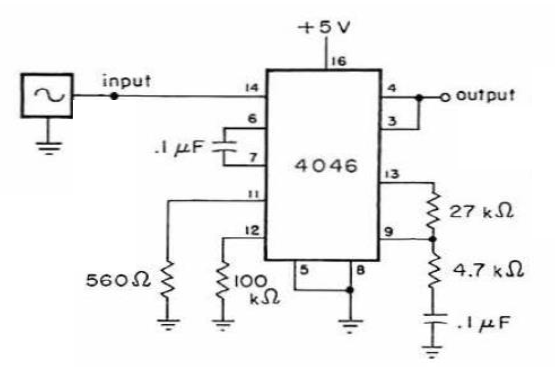
\includegraphics[width= 0.8\textwidth]{../1. PLL/Imagenes/Circuito PLL.png} 
	\label{fig:Circuito PLL}
	\caption{Setup recomendado}
\end{figure}

\subsection{Funcionamiento de un PLL}

Lo que se muestra en la Figura \ref{DiagramaBloquePLL} es un diagrama de bloques de un PLL básico. Se asume que hay una señal de entrada que al ingresar, se la multiplica en un comparador de fase por la salida de un VCO cuya frecuencia, seleccionada en el diseño, es de $f_0$. El producto de la multiplicación es filtrado por un filtro pasa-bajos(LPF) de forma tal que se elimina el ripple y el ruido de alta frecuencia, solo quedando en la salida una tensión proporcional a la diferencia de fase instantánea (la integral de la diferencia de frecuencia) entre las señales multiplicadas. Esta tensión controla la frecuencia del VCO. Si no hay señal en la entrada, no hay voltaje de error a la salida del comparador, por lo que tampoco lo hay a la salida del LPF. En esta situación, el VCO está fijo en su frecuencia central, $f_0$.


\begin{figure}[h!]
	\centering
	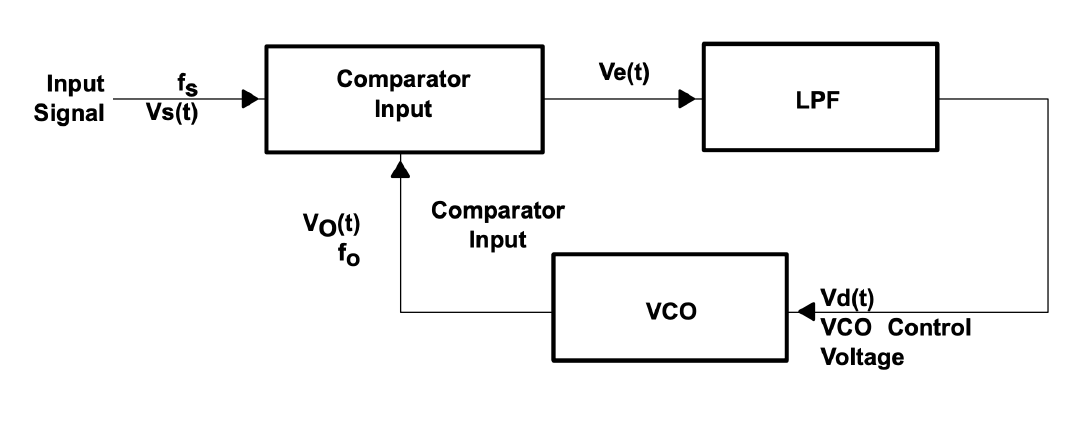
\includegraphics[width=1\textwidth]{../1. PLL/Imagenes/Diagrama bloque PLL.png}
	\caption{Diadrama de bloque de un PLL}
	\label{DiagramaBloquePLL}
\end{figure}

La entrada al VCO varía reduciendo la diferencia de frecuencia entre el VCO y la señal de entrada y a su vez es proporcional a esta diferencia, logrando que la frecuencia del VCO tienda a la frecuencia de la señal de entrada, en otras palabras, realiza un seguimiento de la misma. Cuando se llega a esta condición se dice que el sistema está \textit{"amarrado"}.

\subsubsection{Rango de enganche}

Utilizando un comparador de fase cuya salida es proporcional al seno del ángulo de error de fase, la tensión de error ve, tras pasar por el filtro pasa-bajos, será:

\begin{equation}
	v_e(t) = K_1 f(t)*sin[\phi_i(t)-\phi_o(t)]
	\label{EqVe}
\end{equation}

siendo: 

\begin{equation}
	K_1 = \frac{A_{in}.A_{VCO}}{2}
\end{equation}

Donde $A_{in}$ es la amplitud de la señal de entrada y $A_{VCO}$ es la amplitud de la salida del VCO. $K_1$ representa aquí la ganancia de conversión del comparador de fase, y $f(t)$ es la respuesta al impulso del filtro pasa-bajos. Asumiendo que la frecuencia del VCO es una función lineal de la tensión de error, esta será:

\begin{equation}
	\omega_0 = \omega_c + \frac{d\phi_o}{dt}
\end{equation}

Reemplazando $\frac{d\phi_o}{dt}$ por $K_2.v_e(t)$, donde $K_2$ es la sensibilidadde tensión del VCO(con unidades $\frac{rad}{V.s}$), y reemplazando $v_e$ por \ref{EqVe} se obtiene:

\begin{equation}
	\frac{d\phi_i(t)}{dt} = \frac{d\phi}{dt} +K.f(t)*sin\phi(t)
	\label{eq:DerPhi}
\end{equation}

Donde $K = K_1 K_2 [\frac{rad}{s}]$ y $\frac{d\phi_i(t)}{dt}$ representa la diferencia entre la frecuencia de la señal de entrada y la frecuencia de la portadora, $\Delta\omega_i$. Por lo tanto asumiendo que la ganancia del filtro es 1, la solución de la ecuación \ref{eq:DerPhi} para estado estacionario es:

\begin{equation}
	sin(\phi) = \frac{\Delta\omega_i}{K}
	\label{eq:SinPhi}
\end{equation}

De esta última se deduce que el sistema mantiene el enganche de frecuencias siempre que:

\begin{equation}
	|\Delta\omega_i|< K
	\label{eq:DeltaOmega}
\end{equation}

Esta última ecuación \ref{eq:DeltaOmega} determina el rango del enganche.

\subsubsection{Rango de captura}
El rango de captura es el rango de frecuencias dentro del cual la frecuencia del VCO puede sincronizarse con la
frecuencia de la señal de entrada, partiendo de una situación de asincronismo. Si se tiene un filtro ideal que filtra solo las componentes de alta frecuencia y no atenúa las componentes de baja frecuencia de la señal, los rangos de captura y enganche coinciden. Cuando el filtro no es ideal y se quiere acotar el rango de enganche, reduciendo el ancho de banda del sistema, es muy probable que se vea restringido el rango de captura. Esto es un problema, ya que se dificulta el enganche fuera de condiciones iniciales. Con un rango de captura reducido, si se perturba el circuito y se produce un desenganche, no necesariamente se alcanzará nuevamente el sincronismo aunque la frecuencia de entrada se encuentre dentro del rango de enganche.
Si el sistema se encuentra enganchado la transferencia del lazo no se ve afectada por el circuito LPF. Sino que la transfrencia se ve determinada por K, que define el rango del enganche. Sin embargo cuando el sistema no está enganchado, las frecuencias de las señales de entrada del comparador no son las mismas y el VCO se ve controlado por una tensión de error variable, que puede ser atenuada por el LPF. Esto es equivalente a modificar la ganancia del lazo, y es así como se genera la diferencia entre rango de captura y de enganche. Si expresamos la transferencia del LPF como:

\begin{equation}
F(j\omega) = F_{\omega}e^{j\psi(\omega)}
\end{equation}

Se obtiene que la tensión de error es:

\begin{equation}
v_e(t) = K_1F_{\Delta\omega_i}sin(\Delta\omega_i t)
\end{equation}

El valor pico de la tensión para la frecuencia de captura $\omega_{ic}$ es:

\begin{equation}
	\hat{v_{ec}} = K_1F_{\Delta\omega_{ic}}
	\label{eq:VecPico}
\end{equation}

Por definición al alcanzar la frecuencia de captura el circuito entra en estado estacionario. La tensión de error por estado estacionario es:

\begin{equation}
	V_{ec} = K_1 sin\psi_c
	\label{eq:Vec}
\end{equation}

Igualamos las ecuaciones \ref{eq:VecPico} y \ref{eq:Vec} y reemplazamos en la expresión \ref{eq:DerPhi}, obtuvimos que:

\begin{equation}
	v_{ec} = K_1 \frac{\Delta\omega_i}{K}
	\label{eq:finalVec}
\end{equation}

De esta última expresión se deduce que el rango de captura es $(\omega_i-\omega_c , \omega_i+\omega_c)$, siendo $\omega_c = KF_{\Delta\omega_{ic}}$

\subsubsection{Filtros}

El filtro colocado entre la salida del comparador de fase y la entrada del VCO se puede analizar desde diversas perspectivas para entender su necesidad y función.
En primer lugar, se lo puede ver como un adaptador de la salida del comparador. Dependiendo de la implementación del comparador de fase, se pueden dar dos situaciones, y para ambas un filtro pasa-bajos adecuado es la solución.
Puede ocurrir que la salida del comparador tenga dos frecuencias, $\omega_o - \omega_i$ y $\omega_o + \omega_i$ , de modo que el filtro no deja pasar a la frecuencia más alta. Para ello, la frecuencia principal del filtro debe ser tal que elimine a la mayor frecuencia sin afectar a la menor. Aquí se ve que la frecuencia de corte del filtro, de ser muy pequeña, limita los rangos de captura y de amarre.
Otra posibilidad es que la salida del comparador solo tenga como frecuencia , y el pasa-bajos sea necesario para actuar como promediador, ya que un pasa-bajos puede actuar como integrador, utilizando la relación:

\begin{equation}
	<X> = \frac{1}{T} \int_0^T x(t)dt
\end{equation}

Por otra parte, el filtro es utilizado para evitar que por la presencia de ruido a la entrada del circuito el VCO cambie su frecuencia de oscilación, para lo cual se busca que su frecuencia de corte sea baja. En cuanto a la implementación del filtro, se puede colocar cualquier filtro de tipo pasa-bajos, se analizan los filtros RC y RRC.
Para el tipo de filtro RC la transferencia viene dada por:

\begin{equation}
	F(s)= \frac{1}{1+s\tau_p}
\end{equation}

Donde $\tau_p=R1.C$ como se muestra en la siguiente figura:

\begin{figure}[hbtp]
	\centering
	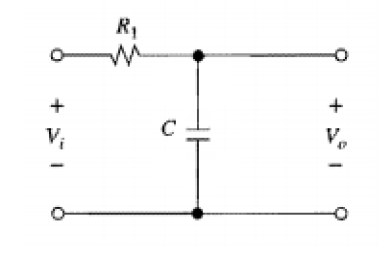
\includegraphics[scale=1]{../1. PLL/Imagenes/Filtro RC.png}
	\caption{Filtro pasa-bajos RC}
	\label{fig:FiltroRC}
\end{figure}

Por lo tanto la transferencia para todo el circuito está dada por:

\begin{equation}
	H(s)= \frac{K/\tau_p}{s^2+ s/\tau_p + K/\tau_p}
	\label{eq:HRC}
\end{equation}

Los parámetros del sistema sub-amortiguado se obtienen de la transferencia y vienen dados por:

\begin{equation}
	\omega_n = \sqrt{K}{\tau_p}
	\label{eq:omeganRC}
\end{equation}

\begin{equation}
	Q = \sqrt{\tau_p K}
	\label{eq:QRC}
\end{equation}

Por otro lado, para el filtro RRC que se muestra en la figura \ref{fig:RRC} se obtiene una transferencia distinta:

\begin{figure}[hbtp]
	\centering
	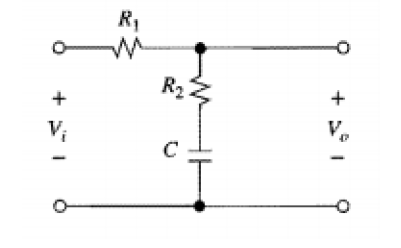
\includegraphics[scale=1]{Imagenes/Filtro RRC.png}
	\caption{Filtro pasa-bajos RRC}
	\label{fig:RRC}
\end{figure}

\begin{equation}
	F(s)= \frac{1 + s \tau_z}{1 + s\tau_p}
	\label{eq:FRRC}
\end{equation}

Donde $\tau_p=(R1+R2)C $ y $\tau_z=R2C$. Si asumimos $R1<<R2$ se aproxima que $\tau_p \approx R2C$. Viendo todo el sistema del PLL se llega a la siguiente transferencia: 

\begin{equation}
	H(s) = \frac{K(s\tau_z +1)(\tau_z+\tau_p) }{ s^2 + s(1+K\tau_z)/\tau_p + K/\tau_p }
	\label{eq:TransRRC}
\end{equation}

Los parámetros del sistema sub-amortiguado se obtienen de la transferencia y vienen dados por:

\begin{equation}
	\omega_n = \sqrt[K]{\tau_p}
	\label{eq:omeganRRC}
\end{equation}

\begin{equation}
	Q = \frac{ \sqrt{K\tau_p} }{ 1 + \tau_z K }
	\label{eq:QRRC}
\end{equation}

En este caso se puede ver que agregando $R2$ se obtiene independencia entre los valores de $Q$ y $\omega_n$ ya que puedo cambiar $Q$, eligiendo un $\tau_z$ conveniente, sin alterar $\omega_n$.



\end{document}